\documentclass{article}
\pdfpagewidth=8.5in
\pdfpageheight=11in

\usepackage{ISRreport}
\usepackage{times}
\usepackage{url}
\usepackage{xcolor}
\usepackage{polski}
\usepackage[polish]{babel}
\usepackage[utf8]{inputenc}
\usepackage[T1]{fontenc}
\usepackage[utf8]{luainputenc}
\usepackage[hidelinks]{hyperref}
\usepackage[utf8]{inputenc}
\usepackage{caption}
\usepackage{indentfirst}
\usepackage{graphicx}
\usepackage{amsmath}
\usepackage{siunitx}
\usepackage{booktabs}
\usepackage{subfig}
\usepackage{pgfplots}
\usepackage{paracol}
\usepackage{gensymb}

\urlstyle{same}
	
\title{Inteligentne Systemy Robotyczne \\ Zadanie sortowania sześcianów}

\author{
Jakub Sikora
\affiliations
numery albumów: 283418 \\
\emails
jakub.sikora2.stud@pw.edu.pl
}

\newcommand{\todo}[1]{\textcolor{red}{\textbf{TO DO:} #1}}

\begin{document}
\maketitle

\section{Opis problemu}
\label{sec:opis-problemu}
\subsection{Treść zadania}
\label{subsec:polecenie}
Należy zaprojektować system sterowania manipulatorem o~sześciu stopniach swobody, wyposażony w~chwytak dwustanowy oraz kamerę RGB-D (Kinect). Na taśmociągu poruszają się różnokolorowe sześciany o~wymiarach 4cm~$\pm$~1cm. Zadaniem robota jest pobieranie żółtych sześcianów poruszających się na czarnym taśmociągu i~układanie ich na palecie o~wymiarach 100cm~x~100cm. Sześciany mają być ustawione na~palecie w~konfiguracji 20x20. 

Szybkość ruchu taśmociągu jest stała i~wynosi $\num{0,1}\frac{m}{s}$ - taśmociąg nie jest sterowany przez projektowany system. Pozycja taśmociągu oraz kamery względem podstawy robota jest znana (określa je projektant systemu). Sześciany spadają pojedynczo na początek taśmociągu co 40~sekund. Ich położenie początkowe i~orientacja są losowe. Szerokość taśmociągu wynosi $\num{0.3}$ m, a~jego długość $\num{1,2}$ m. System rozpoczyna pracę po otrzymaniu komendy \texttt{START}, a~kończy ją gdy paleta się zapełni. Komendy \texttt{START} wydawane są przez zdalnego agenta, którego definiować nie potrzeba. Wymiana palet jest zadaniem innych urządzeń, które nie są pod kontrolą projektowanego systemu.

Stosująć formalizm przedstawiony na wykładzie należy:
\begin{itemize}
    \item określić strukturę systemu w~kategoriach agentów,
    \item dla każdego agenta należy zdefiniować podsystem sterowania, efektory i~receptory wirtualne,
    \item dla tych podsystemów określić:
    \begin{itemize}
        \item automat skończony sterujący ich pracą,
        \item zachowania,
        \item warunki początkowe i~końcowe zachowań,
        \item funkcje przejścia w~postaci matematycznej i~DFD,
        \item zawartość pamięci wewnętrznej oraz buforów wejściowych i~wyjściowych,
        \item krok dyskretyzacji dla każdego podsystemu.
    \end{itemize}
\end{itemize}


\section{Struktura systemu}
\label{sec:struktura}
\subsection{Konfiguracja rzeczywista}
\label{subsec:konfiguracja-urzadzen}

\begin{figure}
    \centering
    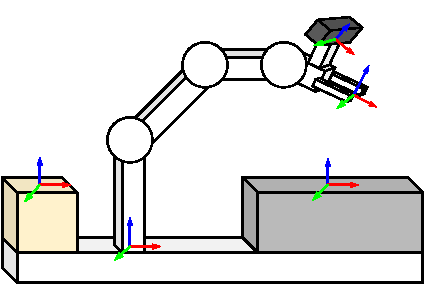
\includegraphics[width=\columnwidth]{figures/ISR-system-overview.pdf}
    \label{fig:srodowisko-robocze}
    \caption{Środowisko robocze projektowanego systemu}
\end{figure}

\subsection{Agentowa struktura systemu}
\label{subsec:agentowa-struktura}

\begin{figure}
    \centering
    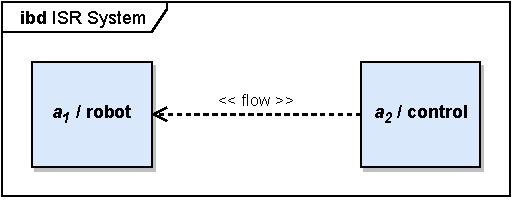
\includegraphics[width=\columnwidth]{figures/ISR-agents.pdf}
    \label{fig:agenty-system}
    \caption{Dekompozycja systemu na agenty}
\end{figure}

\begin{figure}
    \centering
    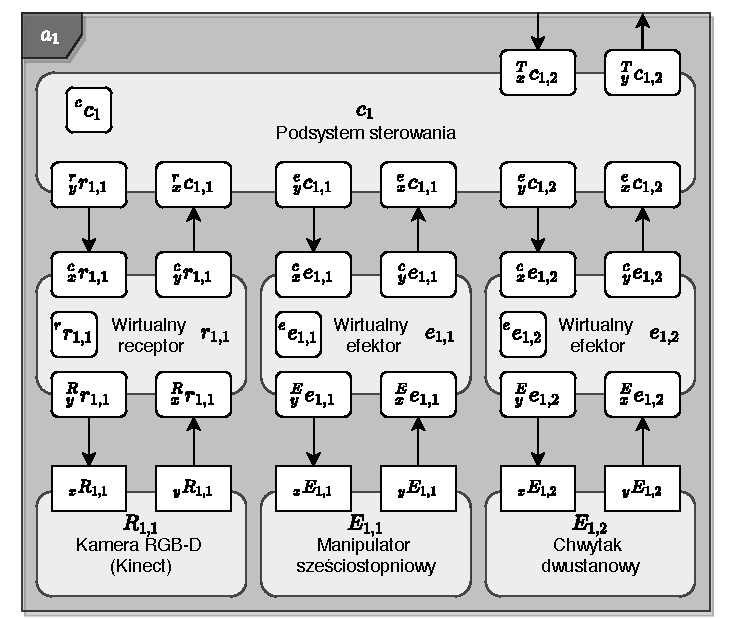
\includegraphics[width=\columnwidth]{figures/ISR-agent-decomposition.pdf}
    \label{fig:dekompozycja-agent-1}
    \caption{Dekompozycja agenta $a_{1}$ na wirtualne i~rzeczywiste receptory i~efektory}
\end{figure}


\todo{Określić niezbędne efektory oraz receptory} \\
Efektory: 
\begin{itemize}
    \item sześciostopniowy manipulator,
    \item chwytak dwustanowy.
\end{itemize}

Receptory:
\begin{itemize}
    \item kamera RGB-D.
\end{itemize}


\todo{Określić liczbę agentów przyporządkowując im efektory i
receptory (wziąć pod uwagę opóźnienia transmisyjne oraz
niezbędną moc obliczeniową)}

Z~faktu iż manipulator jest sześciostopniowy, sterowanie nim nie jest trudne (jest zawsze jedno rozwiązanie problemu kinematyki odwrotnej). Podobnie chwytak dwustanowy, jest albo zamykany albo otwierany więc też lajtowe. Największy problem to kamera RGB-D i analizowanie obrazu. Obraz Kinecta jest w niskiej rozdzielczości 640 x 480 pikseli przy 30 klatkach na sekundę. Przy 30 klatkach na sekundę, przedmioty na taśmociągu przesuną się o 3mm pomiędzy klatkami.

kamera stacjonarna zawieszona nad obszarem roboczym (SAC \emph{Stand Alone Camera}) 

\todo{Określić zachowania każdego z agentów}

Podejrzewam że będą takie zachowania: 
\begin{itemize}
    \item idle,
    \item szukanie sześcianu,
    \item chwytanie,
    \item odkładanie.
\end{itemize}


\todo{Zdefiniować receptory i efektory wirtualne (widoki receptorów
i efektorów oraz bufory komunikacyjne w podsystemie sterowania)}

Slajdy od 141 dalej (wyjebane w kosmos)

Podsystem sterowania (slajdy 125-135): 

Efektor wirtualny manipulatora:
\begin{itemize}
    \item bufor wejściowy od podsystemu sterowania: pozycja pożądana,
    \item bufor wyjściowy do podsystemu sterowania: pozycja aktualna,
    \item bufor wejściowy od rzeczywistego efektora: aktualne położenie wałów silnika,
    \item bufor wyjściowy do rzeczywistego efektora: pożądana pozycja wałów silnika.
\end{itemize}

Efektor wirtualny chwytaka (slajdy 113-119):
\begin{itemize}
    \item bufor wejściowy od podsystemu sterowania: stan pożądany,
    \item bufor wyjściowy do podsystemu sterowania: stan aktualny,
    \item bufor wejściowy od rzeczywistego efektora: stan aktualny,
    \item bufor wyjściowy do rzeczywistego efektora: stan pożądany.
\end{itemize}

Receptor wirtualny kamery RGBD (slajdy 120-122):
\begin{itemize}
    \item bufor wejściowy od rzeczywistego receptora: obraz z kamery,
    \item bufor wyjściowy do podsystemu sterowania
\end{itemize}

\todo{Zdefiniować okres próbkowania dla każdego podsystemu}
Receptor 30 klatek na sekundę daje 33ms.

Efektor czyta wejścia co 1ms natomiast wysyła co 20ms. 


\todo{Zbudować automat skończony przełączający zachowania}

\todo{Zdefiniować warunki początkowe dla poszczególnych zachowań}

\todo{Zdefiniować funkcje przejścia i warunki końcowe dla każdego
zachowania}


\bibliographystyle{abbrv}
\bibliography{bibliography}

\end{document}